\chapter{\label{sec:korr_kapcs}Korrekció a kapcsolófelületen}

\section{Transzverzális metszés, hibrid dinamikai rendszer}

Tekintsük az alábbi hibrid dinamikai rendszert:
%
\begin{equation}
\dot{x}=F(x),
\end{equation}
%
\noindent melynek fundamentális megoldása $\Phi (x,t)$ és
%
\begin{equation}
x \mapsto R(x),
\end{equation}
%
\noindent leképezés a $\sum:=\left\{ x, H(x)=0 \right\} $-n. Kérdés: hogyen számítsuk ki egy olyan periodikus pálya stabilitását, mely "ütközik"?

Jelölje (lásd ábra):
\begin{itemize}
\item $x^*=\Phi(x_p,t_1)$, ahol $x_p$ a periodikus pálya egy pontja
\item $x_0=\Phi(\hat{x},t_1)$, ahol $\hat{x}$ a perturbált pálya egy $x_p$ melletti pontja
\item $x_3=R(\Phi(\hat{x},t_1+\delta))$
\end{itemize}
Keressük azt a $Q(x)$ leképezést, melyre teljesül, hogy
\begin{align*}
x_4=Q(x_0)\,,
\end{align*}
ahol 
\begin{align*}
x_4=\Phi(x_3,-\delta)=\Phi(\overbrace{R(\underbrace{\Phi(x_0,\delta)}_{x_5})}^{x_3},-\delta)\,.
\end{align*}
\begin{figure}[ht]
\centering
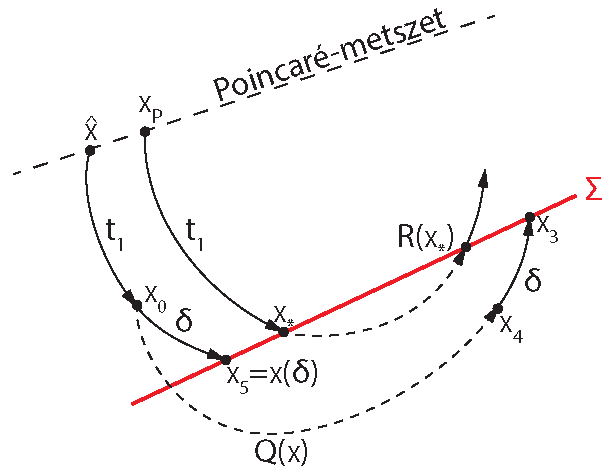
\includegraphics[width=0.5\textwidth]{graphics/korrKapcs1.png}
\caption{Periodikus pálya a kapcsolóvonal közelében.}
\end{figure}

Azaz melyik az a leképezés, amely $\hat{x}$-ból indítva $t_1$-ig (és \emph{nem} $t_1+\delta$-ig) integrálva olyan pontba visz, hogy onnan újabb $\delta$-ig integrálva a helyes $x_3$ pontba érkezünk? Másképp fogalmazva, meghatározandó az a $Q(x)$ leképezés, amely $x_0$ pont $x_4=Q(x_0)$ képéből indulva $\delta$ ideig integrálva ugyanúgy $x_3$-ba visz, mintha $x_5$ pontban alkalmaztuk volna az $R(x)$ leképezést.
\par Tehát meg kell konstruálnunk a $x_0\mapsto Q(x_0)=x_4$ leképezést.
A megoldást $x_0$ körül, kis $\delta$ értékekre sorbafejtve kapjuk, hogy:
%
\begin{equation}
x_5=x(\delta)=\Phi(x_0,\delta)|_{t=0}=x_0+\delta F(x_0)+\mathcal{O}(\delta^2).
\end{equation}
%
Legyen $x_0=x^*+\Delta x$, ezt behelyettesítve a fenti egyenletbe kapjuk, hogy
%
\begin{equation}
x(\delta)=x^*+\Delta x+\underbrace{\delta F(x^*+\Delta x)}_{ F|_{\Delta x=0}= F(x^*)+\underbrace{\Delta x \cdot \textvisiblespace\,}_{\delta \Delta x \approx 0} }+\mathcal{O}(\delta^2)=x^*+\Delta x+\delta F(x^*)+\mathcal{O}(\delta^2,\delta \, \Delta x, \Delta x^2)
\end{equation}
Másrészről, mivel $x_5=x(\delta)$ rajta van a kapcsolófelületen:
%
\begin{equation}
O=H(x(\delta))=H(x^*+\Delta x+\delta F(x^*)+\mathcal{O}(\delta^2,\delta \, \Delta x, \Delta x^2))\,,
\end{equation}
%
valamint $H(x)$ sorfejtése $x^*$ körül 
%
\begin{equation}
H(x)|_{x=x^*}=\underbrace{H(x^*)}_{=0}+H_x(x^*)(x-x^*)+\mathcal{O}(\|{x-x^*}\|^2)\,,
\end{equation}
tehát:
\begin{equation}
O=H_x(x^*)(\Delta x+\delta F(x^*))+\mathcal{O}(2)\,.
\end{equation}

Így $\delta$-ra adódik, hogy:
\begin{equation}
\delta=-\frac{H_x(x^*)\Delta x}{H_x(x^*)F(x^*)}+\mathcal{O}(2)\,,
\end{equation}
amely azt jelenti, hogy a kapcsolófelület $H_x(x)$ gradiensét kell kiértékelni $x^*$ helyen ahhoz, hogy becslést tudjunk adni a szükséges korrekcióra. A becslés hibája $\mathcal{O}(2)$, így a kapcsolófelület ferdeségét figyelembe véve becsülhető a $\delta$ idő, amely alatt a zavart $\hat x$ pontból indított megoldás $t_1$ idő elteltét követően elérte volna a kapcsolófelületet.\par
% <img src="korrKapcs2.png" width="300px"/>
Továbbá:
\begin{align}
x_3&=R(x(\delta))=R(x^*+\Delta x+\delta F(x^*)+\mathcal{O}(2))\,, \\
x_4&=\Phi(x_3,-\delta)|_{t=0}=x_3-\delta F(x_3)+\mathcal{O}(\delta^2) \,,
\end{align}
amiből az $x_4$ az $x^*$ körül:
\begin{multline}
\left.x_4\right|_{x^*}=\underbrace{R(x^*)+R_x(x^*)\overbrace{(\Delta x+\delta F(x^*))}^{-x^*+x(\delta)}}_{x_3}-\delta F\underbrace{(R\overbrace{(x^*+\Delta x+\delta F(x^*))}^{x(\delta)}}_{x_3})+\mathcal{O}(2)=\\
=R(x^*)+R_x(x^*)\Delta x+ \delta [R_x(x^*)F(x^*)-F(R(x^*))]+\mathcal{O}(2)\,.
\end{multline}

Mivel $\Delta x=x_0-x^*$ a keresett $x_0 \mapsto Q(x_0)=x_4$ leképezés, ezért 
\begin{equation}
Q(x_0)|_{x^*}=R(x^*)+R_x(x^*)\Delta x-\frac{H_x(x^*)\Delta x}{H_x(x^*)F(x^*)}(R_x(x^*)F(x^*)-F(R(x^*)))\,,
\label{linearizaltx4}
\end{equation}
%
ahol az $x_0$ aktuális helye  függ az $\hat{ x}$-tól, tehát a perturbáció mértékétől, így $\Delta x$ szintén a zavarástól függ.
 $Q_x$ leképezés szintén linearizálható $x^*$ körül, amely $x_0$ helyen: 
\begin{equation}
Q(x_0)|{x^*}=R(x^*)+Q_x(x^*)\Delta x\,.
\label{linearizaltlekepezes}
\end{equation}
%
Ebből a \ref{linearizaltlekepezes} egyenletben szereplő $Q_x(x^*)$ mátrix meghatározható $\Delta x$ együtthatóinak kigyűjtésével \ref{linearizaltx4} egyenletből:
\begin{equation}
Q_x(x^*)=R_x(x^*)+\frac{F(R(x^*))-R_x(x^*)F(x^*)}{H_x(x^*)F(x^*)}H_x(x^*)\,.
\end{equation}

\section{Példa}
Vegyük a következő folytonos rendszert:
\[F(x) = \left(
\begin{matrix}
x_2\\
-x_1 - 2 \xi x_2 + \mathrm{cos}(\omega t)\\
1
\end{matrix}
\right) = \left(
\begin{matrix}
x_2\\
a\\
1
\end{matrix}
\right),
\]
továbbá a kapcsolóvonal 
$ H(x) =  x_1 - \delta \quad$, vagyis $x_1 = \delta$-nál fal van, így
$ R(x) = \left(x_1,-rx_2,x_3\right)^\mathrm{T} \quad$, melynek $x$ szerinti deriváltja
\[R_x(x) = 
\left(
\begin{matrix}
1 & 0 & 0 \\
0 & -r & 0 \\
0 & 0 & 1
\end{matrix}
\right)\]
\textsl{(Megj.: $\delta$ a levezetések során egy időtartamot jelölt, a feladatbeli jelentése egy távolság.)}\par
A becsapódás normál sebessége: $v = H_x(x^*) F(x^*)=x_2^*$, továbbá jelölje $a^-$ és $a^+$ az ütközés előtti és utáni pillanatbeli értékeket, vagyis
$a^- = -x_{1}^* - 2 \xi x_{2}^* + \mathrm{cos}(\omega t)$ és
$a^+ = -x_{1}^* + 2 \xi r x_{2}^* + \mathrm{cos}(\omega t)$.

Ezekkel:
$ Q_x = 
\underbrace{\left(\begin{matrix}
1 & 0 & 0 \\
0 & -r & 0 \\
0 & 0 & 1
\end{matrix}\right)}_{R_x\left(x^*\right)} +
\underbrace{\frac{1}{v}}_{\frac{1}{H_x\left(x^*\right) F\left(x^*\right)}}
\left(
\underbrace{
\left(
\begin{matrix}
-rv \\
a^+ \\
1
\end{matrix}
\right)}_{F\left(R \left(x^* \right) \right)}-
\underbrace{
\left(
\begin{matrix}
1 & 0 & 0 \\
0 & -r & 0 \\
0 & 0 & 1
\end{matrix}
\right)}_{R_x\left(x^*\right)}
\underbrace{
\left(
\begin{matrix}
v \\
a^- \\
1
\end{matrix}
\right)
}_{F\left(x^*\right)}
\right)
\underbrace{
\left(
\begin{matrix}
1 & 0 & 0
\end{matrix}
\right)
}_{H_x\left(x^*\right)}
= \\
=
\left(
\begin{matrix}
1 & 0 & 0 \\
0 & -r & 0 \\
0 & 0 & 1
\end{matrix}
\right) + \frac{1}{v}
\left(
\begin{matrix}
-rv -v \\
a^+ + ra^- \\
0
\end{matrix}
\right)
\left(
\begin{matrix}
1 & 0 & 0
\end{matrix}
\right)
= \\
=
\left(
\begin{matrix}
1 & 0 & 0 \\
0 & -r & 0 \\
0 & 0 & 1
\end{matrix}
\right) + \frac{1}{v}
\left(
\begin{matrix}
-rv -v & 0 & 0\\
a^+ + ra^- & 0 & 0\\
0 & 0 & 0
\end{matrix}
\right)
=
\left(
\begin{matrix}
-r & 0 & 0\\
\frac{a^+ + ra^-}{v} & -r & 0\\
0 & 0 & 1
\end{matrix}
\right)
$\linebreak
\textsl{(Megj.: A skalár gradiensét (pl. most: $H_x(x))$ sorvektorként értelmezzük, ami egybevág azzal, hogy a Jacobi mátrix sorai is a vektor adott elemének mint skalárnak a gradiensét tartalmazzák)}


\section{Transzverzális metszés, általános eset}

%Itt sokminden le van gépelve, csak ki van kommentelve.

Korrekció a kapcsolósíkon. Az általános esetben:
\[
{\dot{x}} = \begin{cases}
   {\ F}_1(x), & \text{ha } \; H({ x})>0 \\
   {\ F}_2(x), & \text{ha } \; H({ x})<0, 
 \end{cases}
\]


%\begin{wrapfigure}{r}{5cm}
\begin{figure}
	\centering
	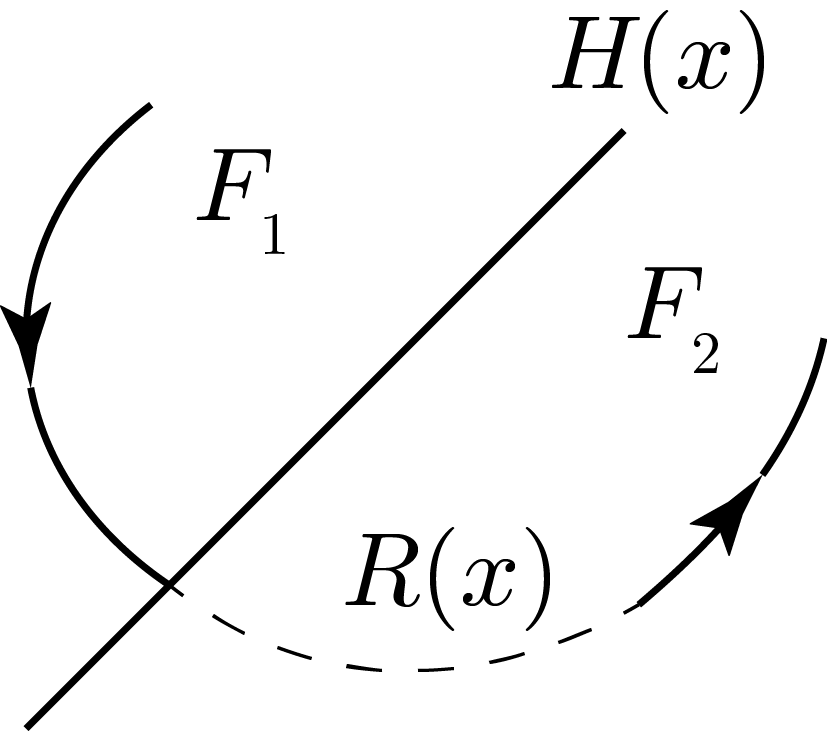
\includegraphics[width=0.35\textwidth]{graphics/5_1.png}
	\caption{$R(x)$ nem kapcsolósíkra képez le.}\label{fig:501}
\end{figure} 
%\end{wrapfigure} 


ahol ${x}\rightarrow R({x}),\; \text{ha}\; H(x)=0.$ Továbbá $R(x)$-nek nem kötelező a kapcsolósíkra leképeznie (lásd \ref{fig:501}. ábra).\\

 A $Q(x)$ korrekciós leképezés alatt a következő érthető: (lásd \ref{fig:502}. ábra)
\noindent
 $\Sigma = \lbrace x,\; H(x)=0 \rbrace,\\
 x^*=\Phi_1(x_p,t),\\
 x_0=\Phi_1{(\hat{x},t_1)} \rightarrow x_2=\Phi_1(x_0,\delta),\\
 x_4=\Phi_2(x_3,-\delta),\\
 x_0 \rightarrow x_4=Q(x_0)=\Phi_2(\underbrace{R(\overbrace{\Phi_1(x_0,\delta)}^{x_2})}_{x_3},-\delta)$

\begin{figure}[ht]
\centering
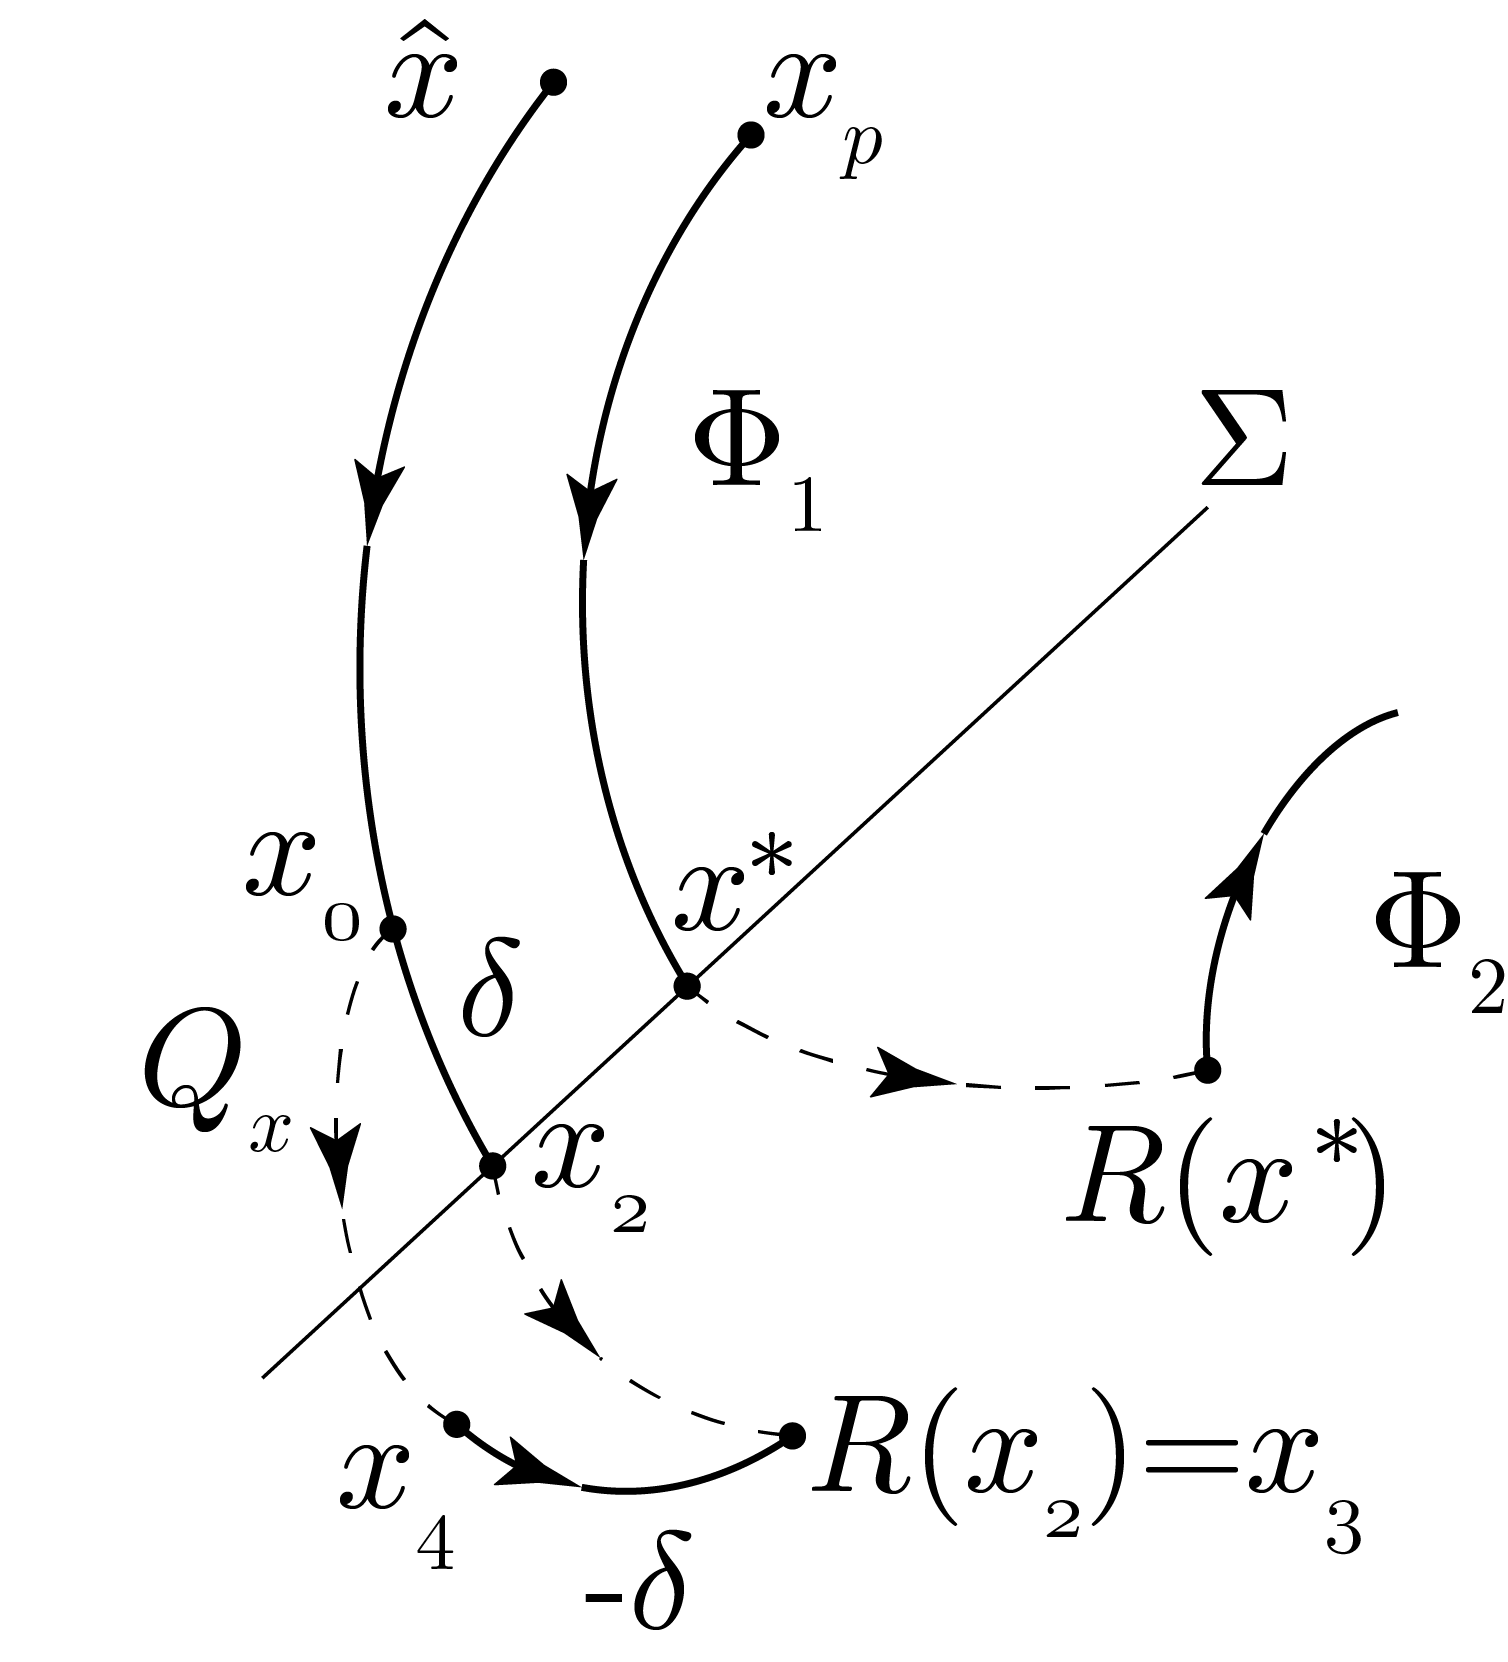
\includegraphics[width=0.4\textwidth]{graphics/5_2.png}
\caption{Korrekció származtatása ha $R(x)$ nem kapcsolósíkra képez le.}\label{fig:502}
\end{figure}

 $Q(x)$ linearizáltjára adódik, hogy:
 \begin{equation}
  Q_x(x^*)=R_x(x^*)+\frac{(F_2(R(x^*))-R_x(x^*)F_1(x^*))H_x(x^*)}{H_x(x^*)F_1(x^*)}
 \end{equation}
  és $H_x(x^*)F_1(x^*)\neq 0$ transzverzális metszés.



 \textbf{Példa 1.)} Filippov rendszer csúszás nélkül, azaz $F_1|_\Sigma \neq F_2|_\Sigma$, valamint $R(x)=x$, azaz önmagába leképezés. \\
 Ilyenkor:
 \[Q_x=I+\frac{(F_2-F_1)H_x}{H_xF_1}, \; \text{mert} \; R(x)=I.\]

 \textbf{Példa 2.)} Ütközéses dinamikai rendszer, ahol $F_1=F_2=F$.
Így $Q(x):$
\[
Q_x(x^*)=R_x(x^*)+\frac{(F(R(x^*))-R_x(x^*)F(x^*))H_x(x^*)}{H_x(x^*)F(x^*)}
\]

 \textbf{Példa 3.)} Filippov rendszer csúszással, azaz
 
 \[
 F_s=F_{12}=(1-\alpha)F_1+\alpha F_2, \; \text{és } \; \alpha=\frac{H_x F_1}{H_x(F_1-F_2)}.
 \]
 Ekkor
\[
	Q_x=F+\frac{(F_{12}-F1)H_x}{H_xF_1}
\]

\begin{figure}[ht]
	\centering
	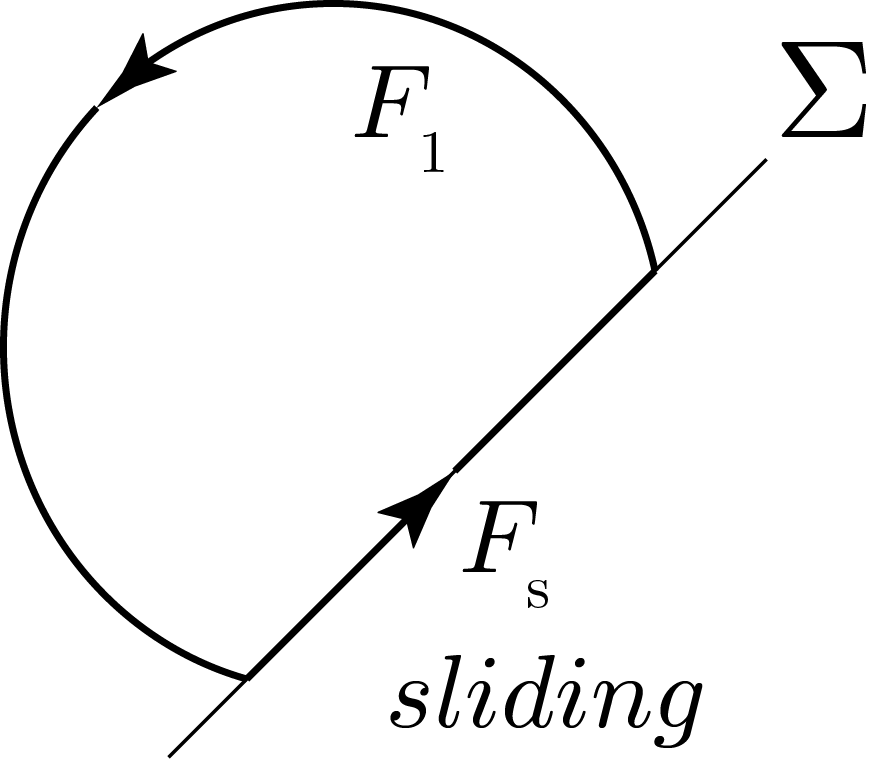
\includegraphics[width=0.4\textwidth]{graphics/5_3.png}
	\caption{Filippov rendszer csúszással}\label{fig:503}
\end{figure}
\clearpage

